%!TEX root = ../Main.tex

\chapter{Introduction}
\label{cha:Introduction}
  Computer graphics are part of most consumer computer systems, such as mobile devices or \glspl{pc}.
  Special purpose hardware, known as \gls{gpu}, is used to accelerate computations related to computer graphics.
  Graphics hardware designs have changed considerably over time.
  In the past, graphics hardware consisted only of fixed-function components that performed necessary computations in a massively parallel manner to transform three-dimensional data to an image that is supposed to be displayed on a screen.
  At the same time, \glspl{api} for this kind of hardware were developed.
  Many modern graphics devices have become more general since then, making them more suitable and accessible to other kinds of computational tasks not directly related to computer graphics.
  Traditional \glspl{api} had to adjust to these changes while maintaining compatibility to previously supported hardware at the same time.
  The result of this is an increase in driver implementation complexity that negatively affects performance at least on the \gls{cpu}.
  New graphics \glspl{api} were designed to match recent hardware more closely.
  One such \gls{api} is the Vulkan graphics API by the \gls{khronos}~\cite{vkspec}, which is presented in this work.


  \section{Document Structure}
    Chapter~\ref{cha:Introduction} is the introduction to the topics discussed within this document.
    In chapter~\ref{cha:VulkanOverview}, an overview of the Vulkan graphics \gls{api} is given in terms of its components and features.
    Chapter~\ref{cha:EnvSetup} is a guide for setting up Vulkan for application development with a bias towards \gls{windows} platforms.
    Chapter~\ref{cha:RenderPipeline} sets up a simple rendering scenario and explains it by showing relevant steps in the form of code samples.
    % And finally, chapter~\ref{cha:Conclusion} concludes this document and provides insight to thoughts of the author about the topics discussed.
    In (chapter~\ref{cha:Conclusion} | the last chapter), remarkable aspects of Vulkan are highlighted and prospects for potential uses of it are presented from the point of view of the author.

  \section{Interaction With Graphics Hardware}
  \label{sec:HardwareInteraction}
    Because \glspl{gpu} are a distinct hardware component in a computer system, \glspl{api} are used to communicate with the \gls{gpu}.
    The level of abstraction an \gls{api} provides varies and depends on the platform and hardware vendor.
    On gaming consoles, for instance, it is common to use graphics \glspl{api} with only minimal abstraction layer, if any, between the application and the \gls{gpu}, allowing applications to take full control of the hardware.
    This is most suitable to systems with a fixed configuration of hardware components.
    On desktop systems, on the other hand, the situation is very different.
    Hardware configurations are rarely the same and change with each release of new graphics hardware, which typically happens more frequently than new gaming consoles are released.
    The situtation for mobile devices is quite similar.
    On such systems, the \glspl{api} tend to define more abstract models that applications will be based on.
    These abstract models are then translated, or mapped, to the actual hardware by the \textit{driver}.
    The relationship between an application and graphics hardware is depicted in figure~\ref{fig:AppApiDriverOverview}.

    \begin{figure}
      \label{fig:AppApiDriverOverview}
      \centering
      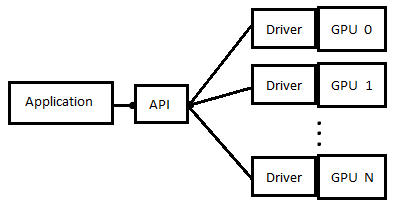
\includegraphics[width=\textwidth]{Main/Images/Application_API_Driver_Overview}
      \caption{Interaction between the application and graphics hardware via an API.}
    \end{figure}


  \section{High Level Graphics Workflow}
    \label{sec:GraphicsWorkflow}
    Generally speaking, graphics hardware is built like a pipeline that is made up of several components called pipeline stages.
    Each of these stages is processing data that is provided by the host application, before being passed on to the next stage in the pipeline.
    The pipeline stages can generally be categorized into fixed-function stages and shader stages.
    Control over the operation of a fixed-function stage is limited, but in many cases they can be configured to some extent.
    Shader stages accept application-defined programs, called \textit{shaders}, that are run in order to process incoming data.
    The terminology used to describe these stages varies between platforms and \glspl{api}.
    In this section, the terms coined by the \gls{khronos} will be used as they are the same as the terms used in the Vulkan specification.

    \begin{figure}
      \label{fig:Rendering_Pipeline_Overview}
      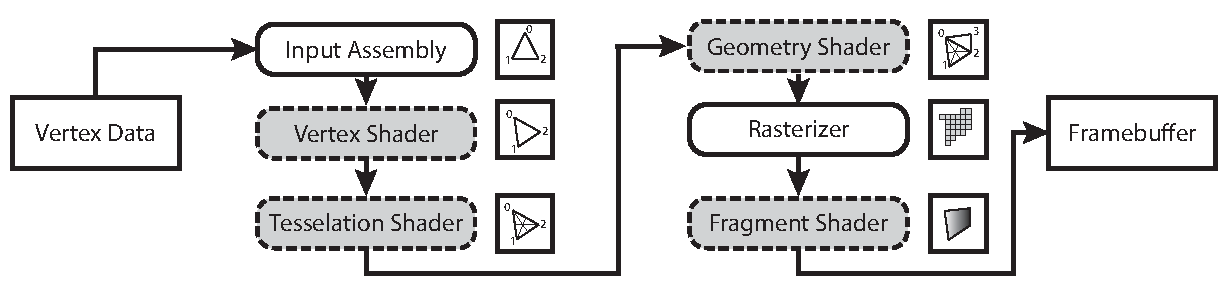
\includegraphics[width=\textwidth]{Main/Images/Rendering_Pipeline_Overview}
      \centering
      \caption{Simplified overview of a graphics pipeline. Fixed-function stages are depicted with solid, rounded outlines and shader stages with dashed outlines.}
    \end{figure}

    Overview of the rendering pipeline on modern graphics hardware is outlined in figure~\ref{fig:Rendering_Pipeline_Overview}.
    It shows all programmable shader stages as well as some fixed-function stages and the flow between them.
    As for the fixed-function stages, only the input assembly and the rasterizer are depicted.
    The input assembly is responsible for assembling vertex data and translating them into primitives such as triangles.
    The rasterizer transforms incoming primitive data in order to produce fragments that will will be processed by the fragment shader to produce pixel values.
    It must be noted that these are just two out of many fixed-function stages.
    A complete list of all pipeline stages can be found in the Vulkan specification chapter~9, specficially figure~9.1~\cite{vkspec}.

    The available shader stages are the vertex, tessellation, geometry, and fragment shader stages.
    Basic functionality and purpose of the shader stages are explained below.

    \begin{description}
      \item[Vertex Shader]
        Vertex shaders are invoked for individual vertices.
        This stage is typically used to transform vertices to different coordinate systems.

      \item[Tessellation Shader]
        Tessellation shaders are used to subdivide geometry using a mathematical function as part of the graphics pipeline.
        This allows applications to reduce the amount of data that is required to be uploaded to the \gls{gpu}.
        For example, this can be used to produce smoother geometry for water surfaces.
        \todo{mention that the tessellation stage consists of two programmable stages and one fixed-function stage in-between?}{}

      \item[Geometry Shader]
        Geometry shaders are used to generate new geometry from existing primitives.
        For example, the geometry shader may be used to turn a single vertex into a triangle.

      \item[Fragment Shader]
        Fragment shaders work on individual output pixels to determine values that are written to the framebuffer.
        In other words, this is the stage where the actual pixel colors are produced, optionally by sampling textures and applying lighting computations.
    \end{description}


  \section{Motivation for a new Graphics API}
    When traditional graphics \glspl{api} were created, they were designed to match hardware architectures that existed at the time.
    However, hardware has changed significantly over time.
    The models employed by traditional graphics \glspl{api} no longer match modern hardware design as closely.
    In order to remain compatible, these \glspl{api} need to perform a mapping of their model to modern hardware design, which may come at a significant cost in terms of performance.

    In practice, this often means that the hardware driver, implementing a traditional graphics \gls{api}, wastes a considerable amount of time that could be used by the host application to perform useful computations.
    For some applications, the additional \gls{cpu} overhead may be acceptable.
    Applications such as these may not gain much by the new \glspl{api} other than lower power consumption due to reduced \gls{cpu} usage, which might be important on mobile platforms.

    Modern hardware design tends to be more suitable for general purpose computing compared to traditional hardware design.
    Graphics hardware consisted of many special purpose components in the past that have largely been replaced by general purpose memory and programmable processing cores that perform work in a massively parallel manner.
    Designing an abstraction that is much closer to modern hardware design allows drivers to work more directly with the hardware and reduce the aforementioned cost of mapping the driver model to the actual hardware.
    This is arguably the main motivation for new graphics \glspl{api} such as Vulkan and \gls{d3d12}.

    Another aspect of modern graphics \glspl{api} is the level of control that is given to the application.
    \glspl{api} such as OpenGL did not allow much control of the hardware itself but rather provided a very abstract model of it.
    Modern \glspl{api}, on the other hand, expose the hardware a lot more.
    The fact that modern graphics hardware has become more general purpose is certainly a factor in this.
    Designing general purpose hardware only to be constrained by \glspl{api} that do not provide ways to leverage it would be a waste of resources.
    % \todo{References??}
    % Additionally, having more control of the hardware has been the desire of many developers in the past.
    On gaming consoles, for example, working closely with graphics hardware has always been possible\footnote{Except on \gls{ms} platforms where \gls{d3d} technology is used.}.
    A game ported from a console to a platform like the \gls{pc} would often run less optimal in comparison in terms of the most optimal use of available resources.

    Providing more control to the application also means that drivers have to do less guess-work to figure out what the application wants to do.
    This makes driver implementations simpler and easier to maintain, reducing the possibility of \glspl{bug}, but it also makes application code more complicated at the same time.
    \todo[fancyline,color=blue!60]{patrigg: the may also optimize api usage for their specific problem --> no additional checks by the driver where this is not needed}
    However, this allows application developers to optimize for different hardware independently of the actual driver implementation.

    Multi-threading is also a concern for modern graphics applications.
    With traditional graphics \glspl{api} it was usually much harder, if not impossible, to utilize multiple threads in terms of rendering.
    At the time these \glspl{api} were designed, applications were usually running only on a single thread.
    Modern graphics \glspl{api}, on the other hand, have been designed with multi-core processing in mind.

    % \todo[inline]{Mention CPU overhead of GPU instructions, especially on mobile.}

    % \todo[inline]{Talk about new APIs such as D3D12, Mantle, Metal, and also talk about consoles (no specs) that all address these problems?}


  \section{The Vulkan Graphics and Compute API}
    The Vulkan \gls{api} was designed by the \gls{khronos} in collaboration with many industry representatives, including Valve Corporation, \gls{amd}, and \gls{nvidia}~\cite{vkspec}.
    Version 1.0 of the Vulkan specification was released on February 16th, 2016~\cite{vkrelease1dot0}.
    It was designed to provide low-level control to the developer when interacting with graphics and compute hardware.

    Vulkan was designed with a variety of goals in mind.

    \begin{description}
      \item[Cross-Platform] Vulkan is supposed to run on multiple platforms that are equipped with different kinds of hardware.
      \item[Reduce Driver Complexity] By relaying more responsibility to the application, driver implementations can be simpler.
      \item[Reduce Driver Overhead] Less driver-side \gls{cpu} overhead.
      \item[Low-level Control] Allow developers a lot of control over the hardware.
      \item[Consistent API] Reduce the amount of new concepts an application developer has to learn when using the \gls{api}.
    \end{description}

    There are many different kinds of hardware configurations today, ranging from high-end gaming systems to mobile platforms such as smartphones.
    Vulkan is designed to be used with all of these systems.
    There will be no special version of Vulkan dedicated to embedded systems as was the case with \gls{gles}.

    As a result of striving for less driver overhead, Vulkan also provides the possibility of reducing \gls{cpu} and \gls{gpu} power consumption.
    The driver implementation will have to make fewer guesses of what the host application is trying to do.
    It is up to the application developer to tell the Vulkan driver exactly what needs to be done.
    This way the driver only does as much work as it needs to function properly and less power will be consumed.
    Hardware vendors will also have an easier time providing robust drivers with less bugs due to reduced complexity.

    Another advantage of Vulkan\todo[fancyline,color=blue!60]{Comma?}{} being a new API built without worrying about backwards compatibility, is the chance of designing a new and consistent API so developers will have an easier time creating applications.
    For more information about the API structure and common patterns in Vulkan, see chapter~\ref{cha:VulkanOverview}.

    Version 1.0 of Vulkan was not entirely built in-house at \gls{khronos} but is in part based on components of AMD's Mantle API, which was donated to the \gls{khronos}~\cite{vksessiongdc15}.


    \subsection{Related APIs}
      There are several other graphics \glspl{api} available for using graphics and compute hardware.
      \gls{opengl} is the predecessor of Vulkan and provides a higher level of abstraction from the hardware.
      It is a very successful API running on several different platforms with varying hardware configurations.
      Due to its level of abstraction, \gls{opengl} drivers are very complex and do a significant amount of work on the \gls{cpu} in order to match abstract commands to the hardware.

      Special flavors of \gls{opengl} exist, such as \gls{gles}, which is a subset of \gls{opengl} to enable hardware-accelerated graphics processing on embedded systems such as smartphones and tablets.

      The \gls{d3d} family of \glspl{api} is developed by Microsoft and only supports Microsoft platforms such as the Windows operating system or the Xbox gaming console.
      The most recent versions of \gls{d3d} are \gls{d3d11} and \gls{d3d12}.
      \gls{d3d11} provides a higher level of abstraction from the hardware than \gls{d3d12}, similar to the relationship between \gls{opengl} and Vulkan.
      It has been around since the release of Windows 7 in 2009.
      \gls{d3d12}, the latest revision of the \gls{d3d} specification released in 2015, is comparable to Vulkan in terms of hardware abstraction.
      It provides much more control to the developer over the hardware.

      Apple developed its own graphics \gls{api} called Metal, which is exclusively available on iOS and Mac OSX platforms.
      Similar to Vulkan and \gls{d3d12}, Metal also offers more direct control over the hardware.

      % Another \gls{api} is OpenCL also developed by the \gls{khronos}.
      % OpenCL only offers a compute \gls{api} and no graphics \gls{api}.
